\documentclass[12pt]{article}

\usepackage[margin=1in]{geometry}
\usepackage{amsmath,amsthm,amssymb}
\usepackage{mathtools}
\usepackage{mathrsfs}
\usepackage{enumitem}
\usepackage{physics}
\usepackage{empheq}
\usepackage{float}
\usepackage{graphicx}
\graphicspath{ {./images/} }

\usepackage{tikz}
\usetikzlibrary{calc,decorations.markings,patterns}

\newcommand{\magsq}[1]{\big|#1\big|^2}
\newcommand{\avg}[1]{\left<#1\right>}
\newcommand{\fullint}{\int_{-\infty}^\infty}
\newcommand{\fullintd}[1]{\fullint\dd#1\:}
\newcommand{\cint}[2]{\int_{#1}^{#2}}
\newcommand{\cintd}[3]{\cint{#1}{#2}\dd#3\:}

\begin{document}

\title{Homework 2}
\author{Sean Ericson \\ Phys 622}
\maketitle

\section*{$0.2.4$ Functional derivative}
\begin{enumerate}[label=(\alph*)]
    \item \;
    \begin{enumerate}[label=(\roman*)]
        \item \[ \lim_{\epsilon\to 0} \frac{1}{\epsilon}\int\dd y \; \left[\phi(y) + \epsilon\delta(y-x) - \phi(y)\right] = \int\dd y \; \delta(y-x) = \boxed{1} \]
        \item
        \begin{align*}
            &\lim_{\epsilon\to 0} \frac{1}{\epsilon}\int\dd y \; \left[\phi^2(y) + 2\epsilon\delta(y-x) + \epsilon^2\delta^2(y-x) - \phi^2(y)\right] \\
            &= \int \dd y \; 2\phi(y)\delta(y-x) \\
            &= \boxed{2\phi(x)}
        \end{align*}
        \item
        \begin{align*}
            &\lim_{\epsilon\to 0} \frac{1}{\epsilon}\int\dd y \; \left[f(\phi(y) + \epsilon\delta(y-x))g(\phi(y) + \epsilon\delta(y-x)) - f(\phi(y))g(\phi(y))\right] \\
            &= \lim_{\epsilon\to 0} \frac{1}{\epsilon}\int\dd y \; \left[\left(f(\phi(y)) + \epsilon\delta(y-x)\dv{f}{\phi}|_{\phi(y)}\right)\left(g(\phi(y)) + \epsilon\delta(y-x)\dv{g}{\phi}|_{\phi(y)}\right) - f(\phi(y))g(\phi(y))\right] \\
            &= \int\dd y \; \left[\delta(y-x)f(\phi(y))\dv{g}{\phi}|_{\phi(y)} + \delta(y-x)g(\phi(y))\dv{f}{\phi}|_{\phi(y)}\right] \\
            &= \boxed{f(\phi(x))\dv{g}{\phi}|_{\phi(x)} + g(\phi(x))\dv{f}{\phi}|_{\phi(x)}}
        \end{align*}
        \item 
        \begin{align*}
            &\lim_{\epsilon\to 0}\frac{1}{\epsilon}\int \dd y\; \left[\left(\dv{y}\left(\phi(y) + \epsilon\delta(y-x)\right)\right)^2 - \left(\dv{\phi}{y}\right)^2\right] \\
            &= \int \dd y\; 2\phi'(y)\delta'(y-x) \\
            &= \boxed{-2\phi''(x)}
        \end{align*}
        \item
        \begin{align*}
            &\lim_{\epsilon\to 0}\frac{1}{\epsilon}\int \dd y\; \left[V(\phi'(y) - \epsilon\delta'(y-x)) - V(\phi'(y))\right] \\
            &= \int \dd y\; \dv{V}{\phi'}|_{\phi'(y)}\delta'(y-x) \\
            &= \boxed{-\dv{x}\dv{V}{\phi'}|_{\phi'(x)}}
        \end{align*}
    \end{enumerate}

    \item We have that
    \begin{align*}
        \delta S &= \int\dd^4x\; \delta\mathscr{L} \\
        &= \int \dd^4x\; \pdv{\mathscr{L}}{\phi}\delta\phi + \pdv{\mathscr{L}}{(\partial_\mu\phi)}\delta(\partial_\mu\phi) \\
        &= \int \dd^4x\; \left(\pdv{\mathscr{L}}{\phi} - \partial_\mu\pdv{\mathscr{L}}{(\partial_\mu\phi)}\right)\delta\phi.
    \end{align*}
    Thus,
    \[ \delta S = 0 \implies \boxed{\pdv{\mathscr{L}}{\phi} - \partial_\mu\pdv{\mathscr{L}}{(\partial_\mu\phi)} = 0.} \]
    Or, using the above definition of the functional derivative,
    \begin{align*}
        & \frac{\delta}{\delta\phi(x)} \int\dd^4y\;\mathscr{L} \\
        &= \lim_{\epsilon\to 0}\frac{1}{\epsilon}\int\dd^4y\; \mathscr{L}(\phi(y) + \epsilon\delta^4(y-x), \partial_\mu\phi(y) + \epsilon\partial_\mu\delta^4(y-x)) - \mathscr{L}(\phi(y), \partial_\mu\phi(y)) \\
        &= \lim_{\epsilon\to 0}\frac{1}{\epsilon}\int\dd^4y\; \mathscr{L}(\phi,\partial_\mu\phi) + \epsilon\pdv{\mathscr{L}}{\phi}\delta^4(y-x) + \epsilon\pdv{\mathscr{L}}{(\partial_\mu\phi)}\partial_\mu\delta^4(y-x) - \mathscr{L}(\phi, \partial_\mu\phi) \\
        &= \int\dd^4y\; \pdv{\mathscr{L}}{\phi}\delta^4(y-x) + \pdv{\mathscr{L}}{(\partial_\mu\phi)}\partial_\mu\delta^4(y-x) \\
        &= \int\dd^4y\; \pdv{\mathscr{L}}{\phi}\delta^4(y-x) -  \partial_\mu\pdv{\mathscr{L}}{(\partial_\mu\phi)}\delta^4(y-x) \\
        &= \pdv{\mathscr{L}}{\phi(x)} - \partial_\mu\pdv{\mathscr{L}}{(\partial_\mu\phi(x))}.
    \end{align*}
    Thus,
    \[ \delta S = 0 \implies \boxed{\pdv{\mathscr{L}}{\phi(x)} - \partial_\mu\pdv{\mathscr{L}}{(\partial_\mu\phi(x))} = 0.} \]
\end{enumerate}


\section*{$0.2.5$ Massive scalar field}
\begin{enumerate}[label=(\alph*)]
    \item Given the derivatives
    \[ \pdv{\mathscr{L}}{\phi} = -\frac{m^2}{2}\phi^*; \quad \pdv{\mathscr{L}}{(\partial_\mu\phi)} = \frac{1}{2}\partial^\mu\phi^*, \]
    \[ \pdv{\mathscr{L}}{\phi^*} = -\frac{m^2}{2}\phi; \quad \pdv{\mathscr{L}}{(\partial_\mu\phi^*)} = \frac{1}{2}\partial^\mu\phi, \]
    the Euler-Lagrange equations are simply
    \[ \boxed{-m^2\phi^* = \partial^2\phi^*; \quad -m^2\phi = \partial^2\phi} \]
    
    \item Nope, this lagrangian is not invariant under a local $U(1)$ transformation:
    \begin{align*}
        \mathscr{L} &\to \frac{1}{2}\left(\partial_\mu\left(\phi e^{i\Lambda}\right)\right)\left(\partial^\mu\left(\phi^* e^{-i\Lambda}\right)\right) - \frac{m^2}{2}\left(\phi e^{i\Lambda}\right)\left(\phi^* e^{-i\Lambda}\right) \\
        &= \frac{1}{2}\left(\left(\partial_\mu \phi\right)e^{i\Lambda} + \left(\partial_\mu e^{i\Lambda}\right)\phi\right)\left(\left(\partial^\mu \phi^*\right)e^{-i\Lambda} + \left(\partial^\mu e^{-i\Lambda}\right)\phi^*\right) - \frac{m^2}{2}\magsq{\phi} \\
        &= \frac{1}{2}\left[\partial_\mu\phi\partial^\mu\phi^* - i\left(\partial_\mu\phi\right)\left(\partial^\mu\Lambda\right)\phi^* + i\left(\partial^\mu\phi^*\right)\left(\partial_\mu\Lambda\right) + \partial_\mu\Lambda\partial^\mu\Lambda\right] - \frac{m^2}{2}\magsq{\phi} \\
        &\neq \frac{1}{2}\partial_\mu\phi\partial^\mu\phi^* - \frac{m^2}{2}\magsq{\phi}
    \end{align*}
\end{enumerate}


\section*{$0.2.6$ Particle in homogeneous $\mathbf{E}$ and $\mathbf{B}$ fields}
\begin{enumerate}[label=(\alph*)]
    \item The force (and hence acceleration) is given by
    \[ \vec{F} = e\left(\vec{E} + \frac{\vec{v}}{c}\times\vec{B}\right) = e\mqty(\frac{B}{c}\dot{y} \\ E_y - \frac{B}{c}\dot{x} \\ E_z)  \]
    \[ \implies \mqty(\ddot{x} \\ \ddot{y} \\ \ddot{z}) = \frac{e}{m}\mqty(\frac{B}{c}\dot{y} \\ E_y - \frac{B}{c}\dot{x} \\ E_z) = \mqty(\omega\dot{y} \\ \frac{e}{m}E_y - \omega\dot{x} \\ \frac{e}{m}E_z)\]
    Looking at just the $z$ components, we see that the motion in that direction is uncoupled from the other two:
    \[ \ddot{z} = \frac{e}{m}E_z \]

    \item From the above expression for the acceleration, we can see that
    \[ \ddot{\xi} = \ddot{x} + i\ddot{y} = \omega\dot{y} + i\left(\frac{e}{m}E_y - \omega\dot{x}\right) = -i\omega\dot{\xi} + i\frac{e}{m}E_y \]
    giving a inhomogeneous ODE for $\xi$ of the form
    \[ \ddot{\xi} + i\omega\dot{\xi} - \frac{e}{m}E_y = 0, \]
    with solution
    \[ \dot{\xi}(t) = Ae^{i\omega t} + \frac{c}{B}E_y \implies \xi(t) = A'e^{i\omega t} + \frac{c}{B}E_yt + B\]
    where $A$, $A'$, and $B$ are complex constants defined by the initial conditions.
    
    \item We have that
    \[ \avg{\vec{v}} = c\vec{E}\times\vec{B}/B^2 = c\frac{E_y}{B}\hat{x}. \]
    Is this really the time-averaged velocity? Let's calculate it:
    \begin{align*}
        \avg{v_x} &= \frac{\omega}{2\pi}\int_0^{2\pi/\omega}\dd t \Re{\dot{\xi}} \\
        &= \frac{\omega}{2\pi}\int_0^{2\pi/\omega}\dd t\; \left[A\cos(\omega t) + c\frac{E_y}{B}\right] \\
        &= \frac{\omega}{2\pi}\frac{2\pi}{\omega}c\frac{E_y}{B} \\
        &= c\frac{E_y}{B} \\
        \avg{v_y} &= \frac{\omega}{2\pi}\int_0^{2\pi/\omega}\dd t \Im{\dot{\xi}} \\
        &\propto \frac{\omega}{2\pi}\int_0^{2\pi/\omega}\sin(\omega t) \\
        &= 0
    \end{align*}
    It is! the time-averaged velocity in the $x-y$ plane is in the $x$-direction, with magnitude $cE_y/B$. If we rearrange this slightly, we see
    \[ \frac{\avg{\vec{v}}}{c} = \frac{E_y}{B}, \]
    so
    \[ \frac{E_y}{B} \ll 1 \implies \frac{\abs{\vec{v}}}{c} \ll 1 \]
    and hence the non-relativisitc approximation is valid.
    
    \item The three qualitatively different trajectories depend on the value of $E_y$ relative to $B$, as seen in Figure 1.
    \begin{figure}[H]
        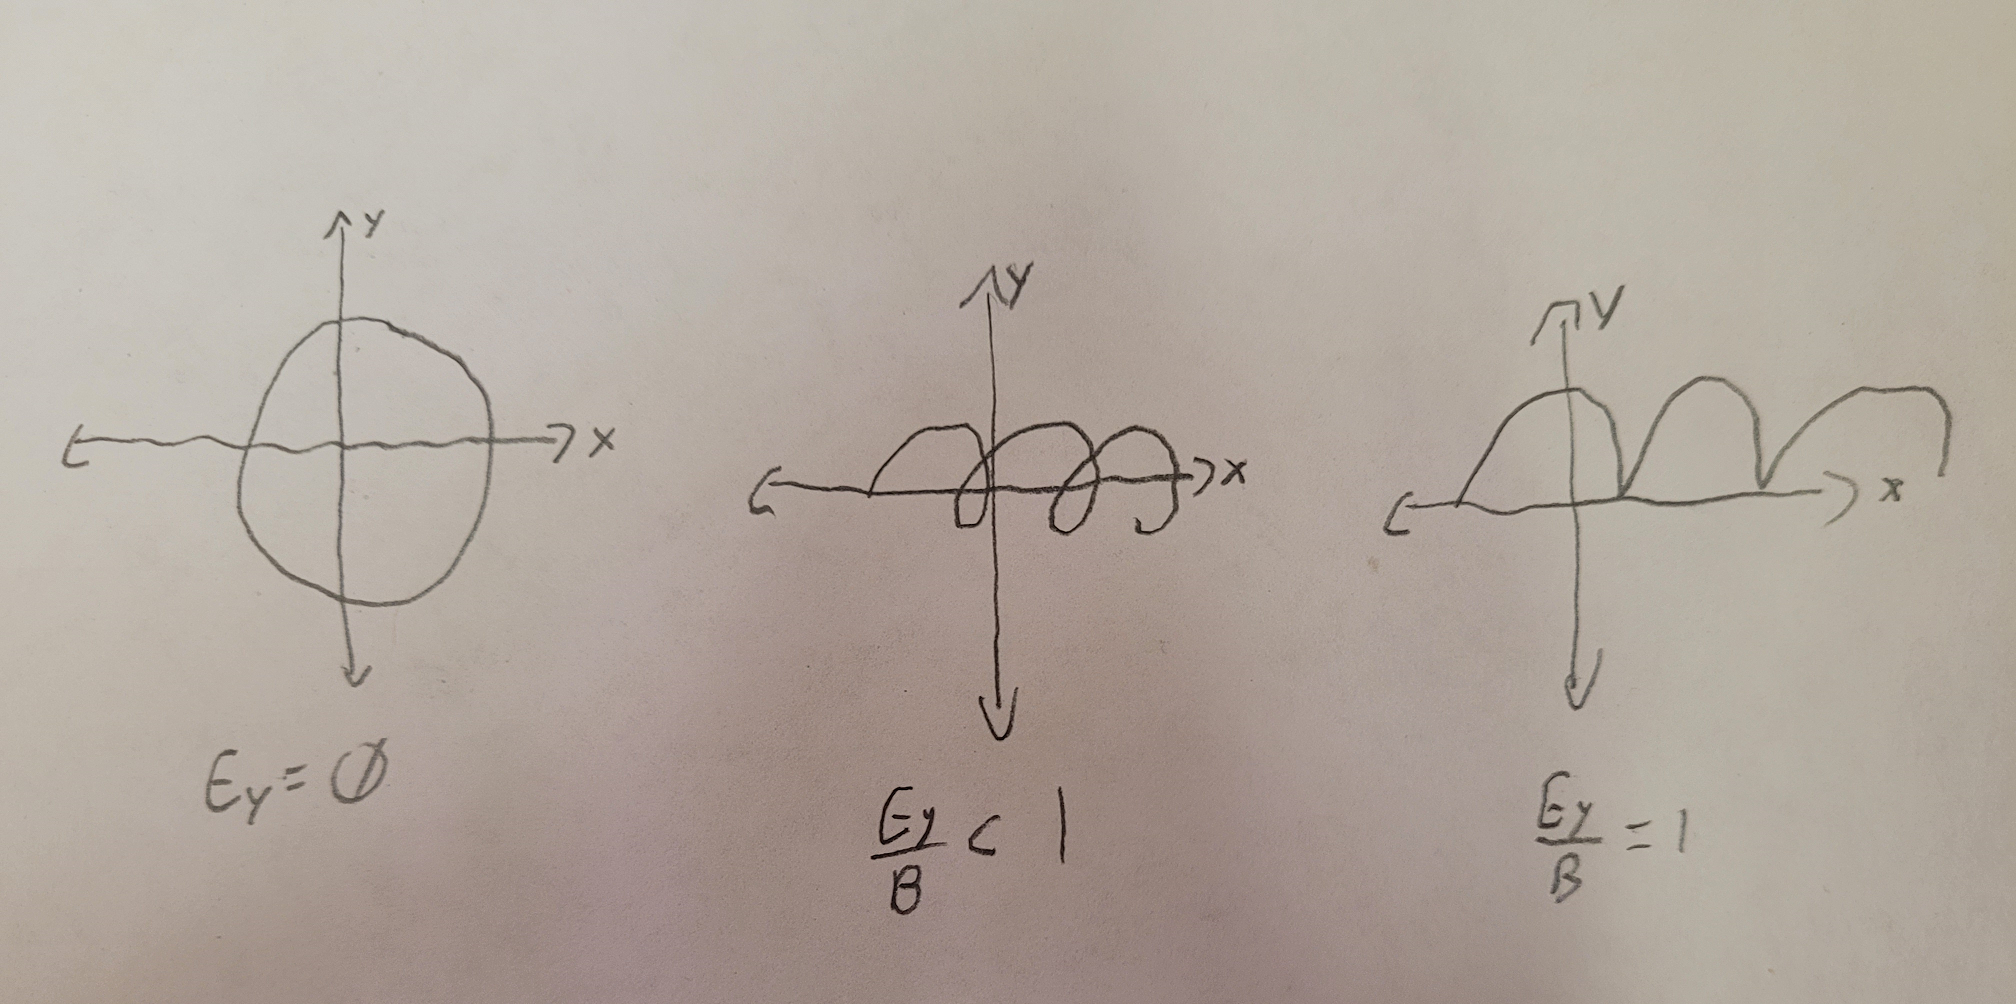
\includegraphics[scale=0.25]{fig1}
        \centering
        \caption{The three qualitatively differnt trajectories.}
        \label{fig1}
    \end{figure}
\end{enumerate}


\section*{$0.2.7$ Harmonic oscillator coupled to a magnetic field}
The force is given by
\begin{align*}
    \vec{F} &= -k\vec{r} + \frac{e}{c}\vec{v}\times\vec{B} \\
    &= -m\omega_0^2\vec{r} + \frac{eB}{c}\dot{y}\hat{x} + \frac{eB}{c}\dot{x}\hat{y} \\
    &= \mqty(-m\omega_0^2 x + m\omega_1\dot{y} \\ -m\omega_0^2y - m\omega_1\dot{x} \\ -m\omega_0^2z)
\end{align*}
where 
\[ \omega_1 = \frac{eB}{mc}. \]
As in the last problem, we can see that motion in the $z$-direction (parallel to $\vec{B}$) decouples from motion in the $x-y$ plane, as
\[ F_z = -m\omega_0^2 z. \]
We can also see that motion is this direction is just that of a 1-dimensional harmonic oscillator with frequency $\omega_0$. \\
Also like the last problem, we can define
\[ \xi = x + iy \]
to help us analyze motion in the $x-y$ plane (the plane perpendicular to $\vec{B}$). From the force above, we can see that the acceleration is
\[ \mqty(\ddot{x} \\ \ddot{y}) = \mqty(\omega_1\dot{y} - \omega_0^2x \\ -\omega_1\dot{x} - \omega_0^2y). \]
In terms of $\xi$, this is 
\[ \ddot{\xi} = -i\omega_1\dot{\xi} - \omega_0^2\xi \implies \ddot{\xi} + i\omega_1\dot{\xi} + \omega_0^2\xi = 0. \]
This is another second-order ODE for $\xi$, with general solution 
\[ \xi(t) = \Re[Ae^{i\tilde{\omega}t}], \]
where $A$ is some complex constant determined by the initial conditions, and
\[ \tilde{\omega} = \frac{1}{2}\left(\sqrt{\omega_1^2 + 4\omega_0^2} - \omega_1\right) \]
is the frequency of oscillation in the plane.

\end{document}